\documentclass[]{standalone}
\usepackage{tikz}
\usepackage{xcolor}
\usepackage{amssymb}
\usepackage{amsmath}
\usepackage{amsfonts}
\usepackage{mathtools}
\usepackage{xspace}
\usepackage{stmaryrd}
\usepackage[misc]{ifsym}
\usepackage{bbold}
\usepackage{etoolbox}

\usepackage[LGR,OT1]{fontenc}
\usepackage[utf8]{inputenc}

\ifcsundef{abf}{\newcommand{\wbf}{\mathbf{w}}
\newcommand{\Wbf}{\mathbf{W}}
\newcommand{\xbf}{\ensuremath{\mathbf{x}}}
\newcommand{\zbf}{\ensuremath{\mathbf{z}}}
\newcommand{\zerobf}{\mathbf{0}}
\newcommand{\h}{h}
\newcommand{\dist}{\mathrm{dist}}

\newcommand{\Acal}{\ensuremath{\mathcal{A}}}
\newcommand{\Bcal}{\ensuremath{\mathcal{B}}}
\newcommand{\Ccal}{\ensuremath{\mathcal{C}}}
\newcommand{\Dcal}{\ensuremath{\mathcal{D}}}
\newcommand{\Fcal}{\ensuremath{\mathcal{F}}}
\newcommand{\Hcal}{\ensuremath{\mathcal{H}}}
\newcommand{\Mcal}{\ensuremath{\mathcal{M}}}
\newcommand{\Ncal}{\ensuremath{\mathcal{N}}}
\newcommand{\Pcal}{\ensuremath{\mathcal{P}}}
\newcommand{\Scal}{\ensuremath{\mathcal{S}}}
\newcommand{\Tcal}{\ensuremath{\mathcal{T}}}
\newcommand{\Xcal}{\ensuremath{\mathcal{X}}}
\newcommand{\Ycal}{\ensuremath{\mathcal{Y}}}
\newcommand{\Zcal}{\ensuremath{\mathcal{Z}}}

\newcommand{\Ebb}{\ensuremath{\mathbb{E}}}
\newcommand{\Pbb}{\ensuremath{\mathbb{P}}}
\newcommand{\Rbb}{\ensuremath{\mathbb{R}}}
\newcommand{\Nbb}{\ensuremath{\mathbb{N}}}

\newcommand{\Rfrak}{\ensuremath{\mathfrak{R}}}

\newcommand{\RA}{\right\rangle}
\newcommand{\LA}{\left\langle}
\newcommand{\LB}{\left[}
\newcommand{\RB}{\right]}
\newcommand{\LC}{\left\{}
\newcommand{\LM}{\left\|}
\newcommand{\RM}{\right\|}
%\newcommand{\RC}{\right\}}
%\newcommand{\RN}{\right\vert}
\newcommand{\LN}{\left\vert}
\newcommand{\LP}{\left(}
\newcommand{\RP}{\right)}

\newcommand{\wrt}{{\it w.r.t.}\xspace}
\newcommand{\eg}{{\it e.g.}\xspace}
\newcommand{\ie}{{\it i.e.}\xspace}
\newcommand{\iid}{{\it i.i.d.}\xspace}

\newcommand{\defeq}{:=}

\DeclareMathOperator*{\EE}{\Ebb}
\DeclareMathOperator*{\PP}{\Pbb}
\DeclareMathOperator*{\argmin}{\mathrm{argmin}}
\DeclareMathOperator*{\vect}{\mathrm{vec}}
\DeclareMathOperator*{\leaky}{\mathrm{Leaky}}
\DeclareMathOperator*{\proj}{\mathrm{Proj}}

\newcommand{\Irm}{\mathrm{I}}
\newcommand{\KL}{\mathrm{KL}}
\newcommand{\KLr}{\overline{\KL}}
\newcommand{\Hell}{H^2}
\newcommand{\TV}{TV}
\newcommand{\kl}{\mathrm{kl}}
\newcommand{\W}{\mathrm{W}}
\newcommand{\Lip}{\mathrm{Lip}}

\newcommand{\D}{\Dcal}
\newcommand{\Dm}{\Dcal_{m}}
\renewcommand{\H}{\Hcal}
\newcommand{\Hb}{\overline{\Hcal}}
\newcommand{\loss}{\ell}
\renewcommand{\P}{\mathrm{P}}
\newcommand{\Q}{\mathrm{Q}}
\newcommand{\R}{\Rbb}
\newcommand{\N}{\Nbb}
\renewcommand{\S}{\Scal}
\newcommand{\Sm}{\S_m}
\newcommand{\Risk}{\text{R}}
\newcommand{\Riskhat}{\hat{\Risk}}
\newcommand{\X}{\Xcal}
\newcommand{\x}{\xbf}
\newcommand{\y}{y}
\newcommand{\Y}{\Ycal}
\newcommand{\Z}{\Zcal}
\newcommand{\z}{\zbf}
\newcommand{\varepsilonbf}{\boldsymbol{\varepsilon}}
\newcommand{\rad}{\mathdbcal{E}}
\newcommand{\DS}{\D_\S}
\newcommand{\yeast}{{\sc Yeast}\xspace}
\newcommand{\phishing}{{\sc Phishing}\xspace}
\newcommand{\mushrooms}{{\sc Mushrooms}\xspace}
\newcommand{\mnist}{{\sc MNIST}\xspace}
\newcommand{\fashion}{{\sc FashionMNIST}\xspace}
\newcommand{\indic}{\mathds{1}}

\newcommand{\OPBTest}{\normalfont\textsc{OPBTest} }
\newcommand{\OPBTrain}{\normalfont\textsc{OPBTrain} }

\newcommand{\Vhat}{\hat{V}}
\newcommand{\Bhat}{\hat{B}}
\DeclareMathOperator*{\ReLU}{\mathrm{ReLU}}

\newcommand{\Cfrak}{\ensuremath{\mathfrak{C}}}

\newcommand{\Poinc}{\texttt{Poinc}}
\newcommand{\Lsob}{\texttt{L-Sob}}
\newcommand{\Ent}{\mathrm{Ent}}
\newcommand{\Var}{\mathrm{Var}}
\DeclareMathOperator*{\Err}{\mathrm{Err}}


\let\oldQ\Q
\let\oldP\P
\renewcommand{\Q}{\orange{\oldQ}}
\renewcommand{\P}{\green{\oldP}}
}{}
%
%%%%%%%%%%%%%%%%%%%%%%%%%%%%%%%%%%%%%%%%%%%%%%%%%%%%%%%%%%%%%%%%%%%%%%%%%%%%%%%
% font option
\renewcommand*\familydefault{\sfdefault}
\DeclareMathAlphabet{\mathgtt}{LGR}{cmtt}{m}{n}

%%%%%%%%%%%%%%%%%%%%%%%%%%%%%%%%%%%%%%%%%%%%%%%%%%%%%%%%%%%%%%%%%%%%%%%%%%%%%%%
% xcolor options

% Paul Tol's  "Vibrant" color scheme
% https://personal.sron.nl/~pault/data/colourschemes.pdf
\definecolor{blue}{HTML}{0077BB}
\definecolor{cyan}{HTML}{33BBEE}
\definecolor{green}{HTML}{009988}
\definecolor{orange}{HTML}{EE7733}
\definecolor{red}{HTML}{CC3311}
\definecolor{magenta}{HTML}{EE3377}
\definecolor{grey}{HTML}{BBBBBB}

%%%%%%%%%%%%%%%%%%%%%%%%%%%%%%%%%%%%%%%%%%%%%%%%%%%%%%%%%%%%%%%%%%%%%%%%%%%%%%%


\begin{document}
\begin{tikzpicture}[thick,scale=0.65, every node/.style={scale=0.65}]

\node[] at (-2,0) {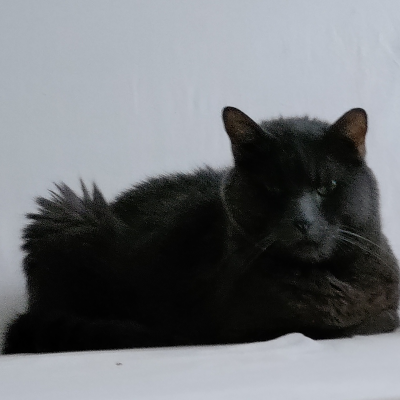
\includegraphics[scale=0.06]{introduction/figures/supervised_cat_1.png}};
\node[] at (-2,1.5) {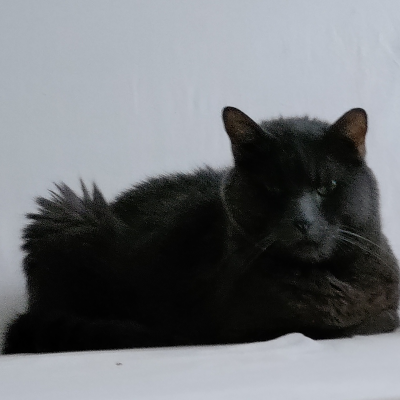
\includegraphics[scale=0.06]{introduction/figures/supervised_cat_1.png}};
\node[] at (-2,3.0) {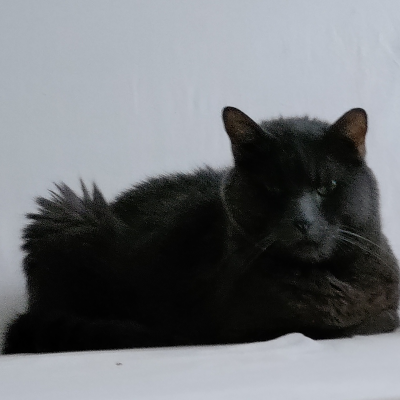
\includegraphics[scale=0.06]{introduction/figures/supervised_cat_1.png}};

\draw[->, line width=0.05cm] (-1.3, 0) -- (0.8, 0);
\draw[->, line width=0.05cm] (-1.3, 1.5) -- (0.8, 1.5);
\draw[->, line width=0.05cm] (-1.3, 3.0) -- (0.8, 3.0);

\node[] at (1.5,0) {
\includegraphics[scale=1.5]{introduction/figures/voter.pdf}};
\node[] at (1.5,1.5) {
\includegraphics[scale=1.5]{introduction/figures/voter.pdf}};
\node[] at (1.5,3.0) {
\includegraphics[scale=1.5]{introduction/figures/voter.pdf}};

\draw[->, line width=0.05cm] (2.2, 0) -- (4.3, 0);
\draw[->, line width=0.05cm] (2.2, 1.5) -- (4.3, 1.5);
\draw[->, line width=0.05cm] (2.2, 3.0) -- (4.3, 3.0);

\node[] at (5.0, 3.0) {\red{Cat}};
\node[] at (5.0, 1.5) {\red{Cat}};
\node[] at (5.0, 0.0) {\blue{Horse}};

\node[] at (1.5, 3.6) {\small Voter 1};
\node[] at (1.5, 2.1) {\small Voter 2};
\node[] at (1.5, 0.6) {\small Voter 3};

\node[rotate=90] at (5.8, 1.5) {$\underbrace{\phantom{aaaaaaaaaaaaaaaaaaaaaaa}}_{}$};

\node[inner sep=0pt] at (7.1, 1.8) {\small Majority vote};
\draw[->, line width=0.05cm] (6.0, 1.5) -- (8.5, 1.5);

\node[] at (9.0, 1.55) {\red{Cat}};

\end{tikzpicture}
\end{document}
